\documentclass[a4paper]{article}

%% Language and font encodings
\usepackage[french]{babel}
\usepackage[utf8x]{inputenc}
\usepackage[T1]{fontenc}

%% Sets page size and margins
\usepackage[a4paper,top=3cm,bottom=3cm,left=2cm,right=2cm,marginparwidth=2cm]{geometry}

%% Useful packages
\usepackage{amsmath}
\usepackage{graphicx}
\usepackage[colorinlistoftodos]{todonotes}
\usepackage[colorlinks=true, allcolors=black]{hyperref}
\usepackage{fourier-orns}
\usepackage{titlesec}
\usepackage{fancyhdr}
\usepackage{fancyvrb}
\usepackage{float}
\pagestyle{fancy} 
\setcounter{tocdepth}{5}

%% Tikz stuff
\usepackage{tikz}
\usetikzlibrary{calc, arrows}
\tikzstyle{incolore} = [rectangle, rounded corners, draw=black, minimum height=1cm, minimum width=3cm, text width=3cm, text centered]

\usepackage{libertine}
\newcommand{\hsp}{\hspace{20pt}}
\newcommand{\HRule}{\rule{\linewidth}{0.5mm}}

\renewcommand{\headrulewidth}{1pt}
\fancyhead[C]{} 
\fancyhead[L]{}
\fancyhead[R]{\footnotesize{\leftmark}}

\renewcommand{\footrulewidth}{1pt}
\fancyfoot[C]{}
\fancyhead[L]{}
\fancyfoot[R]{\thepage}

\definecolor{Zgris}{rgb}{0.87,0.85,0.85}

\usepackage{eso-pic,graphicx}
\usepackage{xcolor}
\newcommand{\bgimg}[1]
{
    \AddToShipoutPicture
    {
        \put(\LenToUnit{0 cm},\LenToUnit{0 cm})
        {
            \includegraphics[width=\paperwidth,height=\paperheight]{#1}
        }
    }
}
\begin{document}





\begin{titlepage}
    \begin{sffamily}
        \begin{center}
            
\includegraphics[width=5cm]{images/LogoHenallux.PNG}~\\[1.5cm]
            \textsc{\Large Rapport de laboratoire}\\[1.5cm]

            % Title
            \HRule \\[0.4cm]
            { \huge \bfseries Septième laboratoire : Simulation de la modulation
            d'amplitude d'un signal analogique \\[0.4cm] }
            \HRule \\[2cm]

            % Author and supervisor
            \begin{minipage}{0.4\textwidth}
                \begin{flushleft} \large
                    Roumache Grégoire\\
                    Sénéchal Julien\\
                    Robert Alexandre\\
                    Wallemme Maxime\\
                    Kenmeugne Lionel\\
                    Didion Charles
                \end{flushleft}
            \end{minipage}
            \begin{minipage}{0.55\textwidth}
                \begin{flushright} \large
                    Laboratoire de sciences appliquées à l'informatique\\
                    Sécurité des systèmes, technologie de l'informatique\\
                    Hénallux\\
                    Première année, groupe H \\
                    Année académique 2019-2020\\
                \end{flushright}
            \end{minipage}
            \vfill

            % Bottom of the page
            {\large 23 Avril 2020}
        \end{center}
    \end{sffamily}
\end{titlepage}







\let\cleardoublepage\clearpage















\section{Introduction}





Dans ce laboratoire, nous avons utilisé le logiciel \textit{NI LabVIEW 2018} pour étudier la modulation de signaux. Nous avons dû refaire le \textit{block-diagram} présent dans l'énoncé de la manipulation et qui équivaut à un code de language de programmation. Nous avons aussi dû ajouter des éléments au \textit{front-panel} qui est une simulation de hardware avec, notamment, des boutons et des panneaux d'affichage.















\section{Rappels théoriques}





La modulation d'amplitude est une technique qui sert à transmettre une information de fréquence peu élevée en modulant l'amplitude d'un signal de fréquence plus élevée. Le signal de fréquence élevée est appelé signal porteur et le signal de fréquence faible est appelé signal modulant.

\begin{figure}[H]
    \centering
    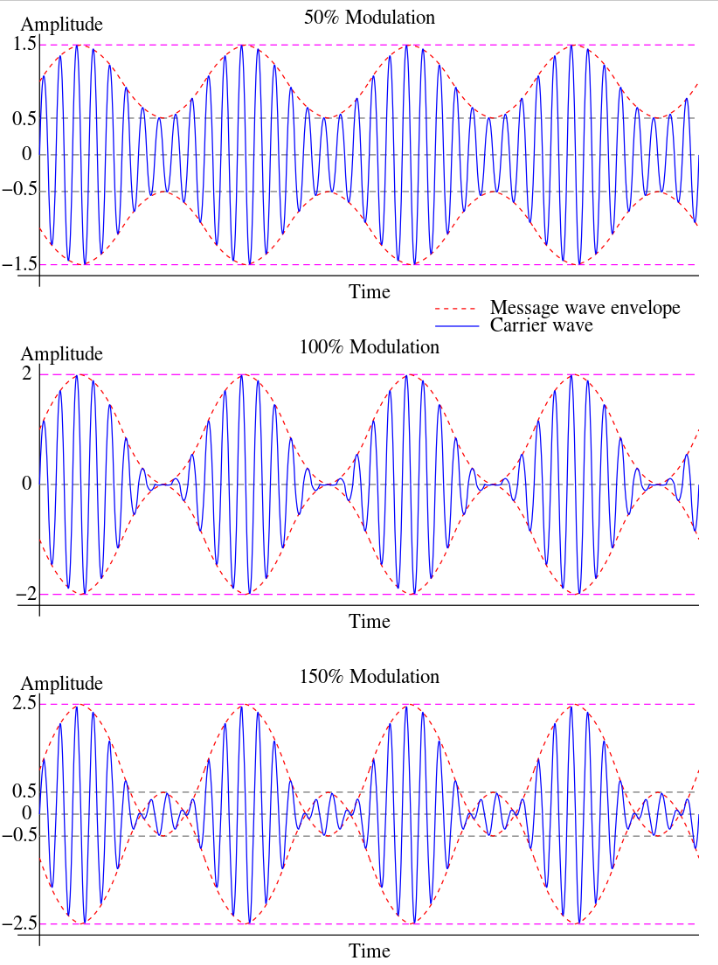
\includegraphics[width=0.65\textwidth]{images/modulation-th-01.PNG}
    \caption{Indice de modulation}
    \label{indiceModulation}
\end{figure}

L'indice de modulation visualisé sur la figure \ref{indiceModulation} est la mesure de la variation d'amplitude par rapport à l'amplitude de la porteuse non modulée. Lorsqu'il est supérieur à 1 (100 \%), le signal est dit \textit{surmodulé}.













\section{Manipulation pratique}





Pour la manipulation, nous avons commencé par télécharger et installer le logiciel \textit{NI LabVIEW 2018} et essayer de comprendre comment ouvrir les fenêtres de \textit{block diagram} et de \textit{front-panel}. Rien que cette étape a pris plusieurs heures car le logiciel fait plusieurs gigaoctets et que l'interface n'était pas simple et claire.

Une fois les fenêtres \textit{block diagram} et \textit{front-end} ouvertes, nous avons ajouté élément par élément la totalité du diagramme qu'il était demandé de reconstituer. Pour l'exemple, nous avons ajouté la figure \ref{fig:f1} pour illustrer l'ajout d'un simulateur de signal dans le \textit{block diagram}. L'entièreté du block diagram est montrée sur la figure \ref{fig:f2}.

\begin{figure}[H]
    \centering
    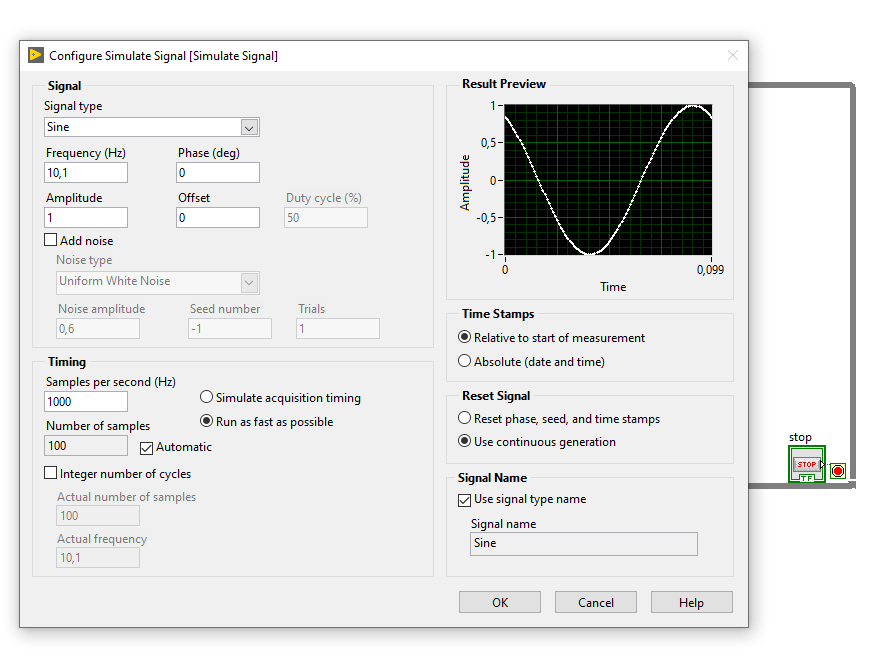
\includegraphics[width=0.99\textwidth]{images/Capture001.PNG}
    \caption{Ajout d'un simulateur de signal}
    \label{fig:f1}
\end{figure}

\begin{figure}[H]
    \centering
    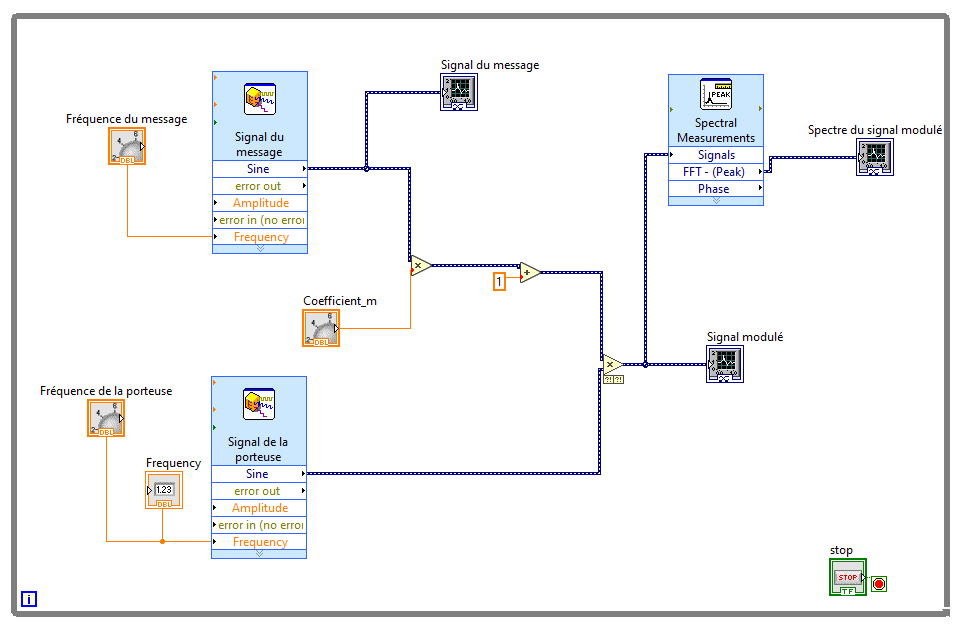
\includegraphics[width=0.99\textwidth]{images/Capture003.PNG}
    \caption{Block diagram complet}
    \label{fig:f2}
\end{figure}





Pour ce qui est du \textit{front-end}, nous avons importés les éléments nécessaires à l'étude de la modulation comme demandé dans l'énoncé de la manipulation, on peut le voir sur la figure \ref{fig:f3}. Ensuite, sur la figure \ref{fig:f4}, on peut voir la même chose mais l'échelle de la fréquence du spectre du signal modulé a été modifiée pour pouvoir mieux le visualiser.

\begin{figure}[H]
    \centering
    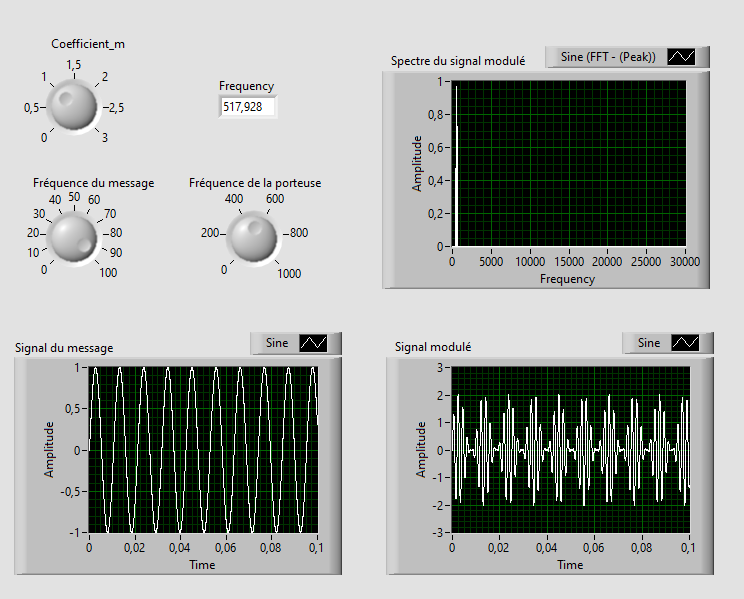
\includegraphics[width=0.99\textwidth]{images/Capture002.PNG}
    \caption{Front-panel avec l'échelle par défaut du spectre du signal modulé}
    \label{fig:f3}
\end{figure}

\begin{figure}[H]
    \centering
    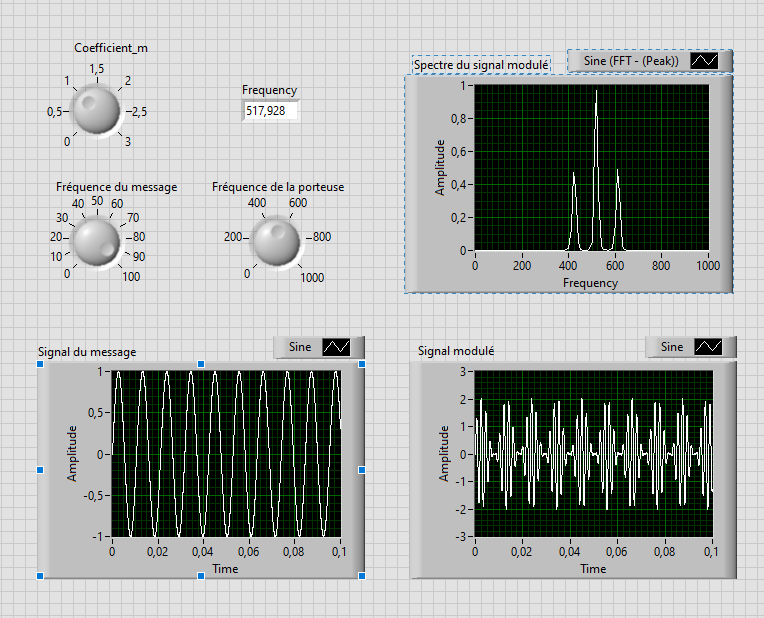
\includegraphics[width=0.99\textwidth]{images/Capture004.PNG}
    \caption{Front-panel avec une échelle adaptée pour le spectre du signal modulé}
    \label{fig:f4}
\end{figure}





Ensuite, nous avons ajouté la figure \ref{fig:f5} qui sert à comparer les signaux porteurs avant et après la modulation. Et finalement, sur la figure \ref{fig:f6}, nous avons tournés tous les boutons au maximum et, notamment, le coefficient de modulation a une valeur de 3, le signal est donc surmodulé.

\begin{figure}[H]
    \centering
    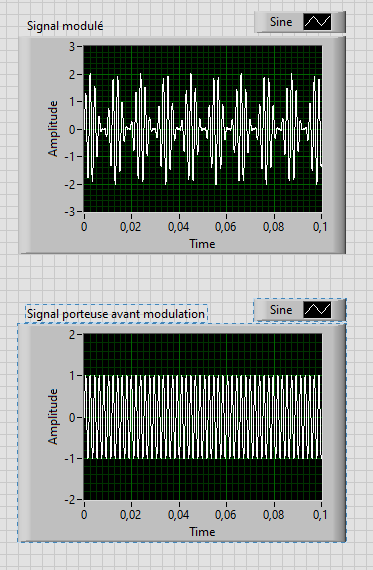
\includegraphics[width=0.70\textwidth]{images/Capture005.PNG}
    \caption{Comparaison signal porteuse avant la modulation et après la modulation}
    \label{fig:f5}
\end{figure}

\begin{figure}[H]
    \centering
    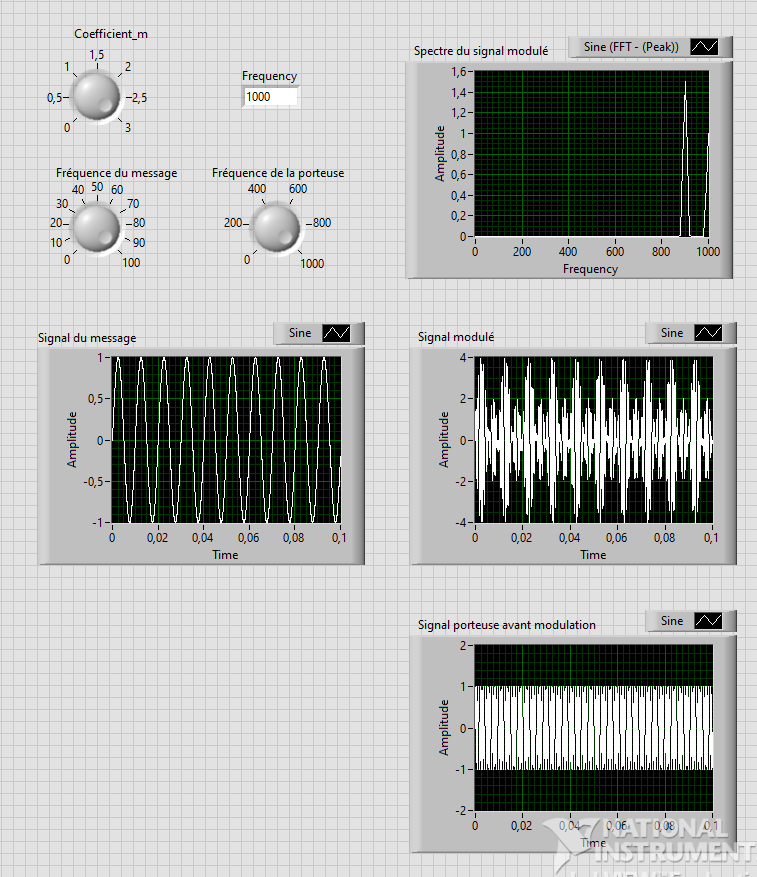
\includegraphics[width=0.99\textwidth]{images/Capture006.PNG}
    \caption{Front-panel après avoir tourné les boutons de gestion de fréquence au maximum}
    \label{fig:f6}
\end{figure}













\section{Conclusion}





Dans ce laboratoire, nous avons appris à utiliser certains aspects du logiciel LabVIEW et nous avons vu et vérifier la théorie de la modulation d'amplitude en insistant sur la surmodulation et le coefficient de modulation, le spectre de fréquence du signal modulé et nous avons visualisé le signal modulé en comparaison du signal porteur et du signal modulant.














\newpage \tableofcontents \listoffigures
\begin{thebibliography}{9}

\bibitem{1} https://fr.wikipedia.org/wiki/Modulation\_d\%27amplitude
\bibitem{2} https://upload.wikimedia.org/wikipedia/commons/thumb/b/b0/Amplitude\_Modulated\_Wave-hm-64.svg/\\
800px-Amplitude\_Modulated\_Wave-hm-64.svg.png
% \bibitem{3} https://fr.wikipedia.org/wiki/Signal\_triangulaire
% \bibitem{4} https://fr.wikipedia.org/wiki/S\%C3\%A9rie\_de\_Fourier
% \bibitem{5} https://en.wikipedia.org/wiki/Fourier\_series

\end{thebibliography}




















\end{document}
